\documentclass[aspectratio=169,11pt]{beamer}

% %% Flowchart styling
\usepackage{tikz}
\usepackage{array}
\usetikzlibrary{arrows.meta,positioning}

\usetheme{Madrid}
\definecolor{uniblue}{RGB}{0,51,102}
\tikzset{
  pipeline step/.style={
    rectangle, rounded corners=3pt, draw=uniblue, thick,
    fill=uniblue!5, text=uniblue, align=center,
    text width=12cm, minimum height=0.8cm,
    inner sep=4pt, font=\small
  },
  pipeline arrow/.style={-{Stealth[length=2mm]}, thick, uniblue}
}
\setbeamercolor{background canvas}{bg=white}
\setbeamercolor{structure}{fg=uniblue}
\setbeamercolor{frametitle}{bg=uniblue,fg=white}
\setbeamercolor{item}{fg=uniblue}
\setbeamercolor{footline left}{bg=uniblue!90!black,fg=white}
\setbeamercolor{footline center}{bg=uniblue,fg=white}
\setbeamercolor{footline right}{bg=uniblue!90!black,fg=white}
\setbeamerfont{footline}{size=\scriptsize}
\setbeamertemplate{navigation symbols}{}
\setbeamertemplate{footline}{%
  \leavevmode%
  \hbox{%
    \begin{beamercolorbox}[wd=.34\paperwidth,ht=2.2ex,dp=1ex,center]{footline left}%
      \usebeamerfont{footline}\insertshorttitle
    \end{beamercolorbox}%
    \begin{beamercolorbox}[wd=.33\paperwidth,ht=2.2ex,dp=1ex,center]{footline center}%
      \usebeamerfont{footline}\insertshortsubtitle
    \end{beamercolorbox}%
    \begin{beamercolorbox}[wd=.33\paperwidth,ht=2.2ex,dp=1ex,center]{footline right}%
      \usebeamerfont{footline}\insertshortdate\hspace{1.2em}\insertframenumber{} / \inserttotalframenumber
    \end{beamercolorbox}%
  }%
}

% %% Presentation title
\title{Acrambly: Perception}
\subtitle{Mid-term Presentation}
\author{}
\date{Oct 2 2026}
\setbeamercolor{title}{bg=uniblue,fg=white}

\begin{document}

\begin{frame}[plain]
  \centering
  \vfill
  \begin{beamercolorbox}{title}
    \parbox[c][1.5cm][c]{\textwidth}{\centering\usebeamerfont{title}\inserttitle}
  \end{beamercolorbox}
  \vspace{0.45cm}
  {\usebeamerfont{subtitle}\insertsubtitle\par}
  \vspace{0.9cm}
  {\usebeamerfont{date}\insertdate\par}
  \vfill
\end{frame}

% %% Presentation outline
\begin{frame}{Outline}
  \vspace{0.45cm}
  {\Large\color{uniblue}
    \setbeamertemplate{enumerate item}{%
      \tikz[baseline=(number.base)]\node[circle,fill=uniblue,text=white,font=\scriptsize,minimum size=0.46cm,inner sep=0pt] (number) {\insertenumlabel};%
    }
    \begin{enumerate}
      \item \textcolor{uniblue}{Perception pipeline 1: White}\vspace{0.42cm}
      \item \textcolor{uniblue}{Perception pipeline 2: Blue}\vspace{0.42cm}
      \item \textcolor{uniblue}{Storage Red}\vspace{0.42cm}
      \item \textcolor{uniblue}{CRAM and RoboKudo integration}
    \end{enumerate}
  }
\end{frame}

\section{White}

% %% White pipeline flowchart
\begin{frame}{Perception Pipline 1: White (1/2)}
  \centering
  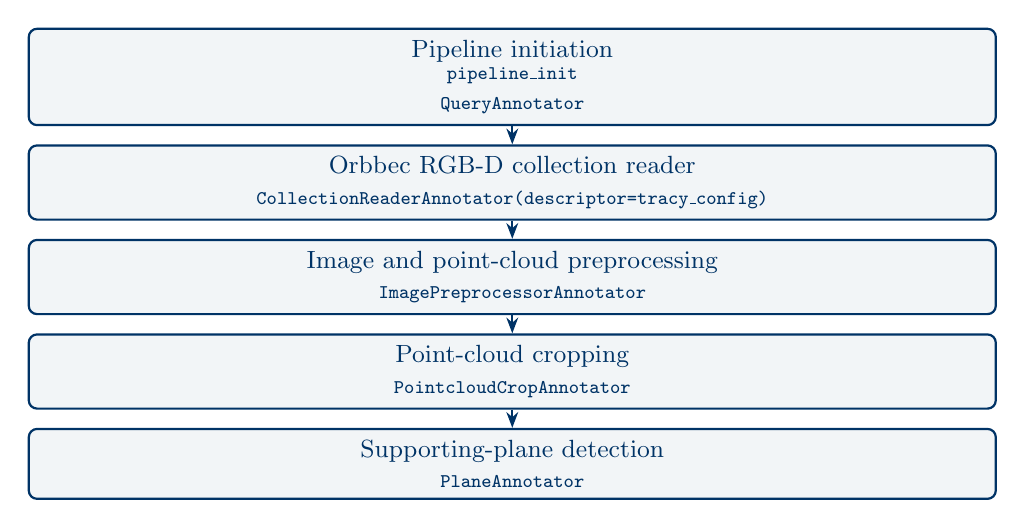
\begin{tikzpicture}[node distance=0.23cm]
    \node[pipeline step] (initiation) {Pipeline initiation\\
      {\scriptsize\texttt{pipeline\_init}\\\texttt{QueryAnnotator}}};
    \node[pipeline step, below=of initiation] (reader) {Orbbec RGB-D collection reader\\
      {\scriptsize\texttt{CollectionReaderAnnotator(descriptor=tracy\_config)}}};
    \node[pipeline step, below=of reader] (preprocessing) {Image and point-cloud preprocessing\\
      {\scriptsize\texttt{ImagePreprocessorAnnotator}}};
    \node[pipeline step, below=of preprocessing] (cropping) {Point-cloud cropping\\
      {\scriptsize\texttt{PointcloudCropAnnotator}}};
    \node[pipeline step, below=of cropping] (plane) {Supporting-plane detection\\
      {\scriptsize\texttt{PlaneAnnotator}}};
    \draw[pipeline arrow] (initiation) -- (reader);
    \draw[pipeline arrow] (reader) -- (preprocessing);
    \draw[pipeline arrow] (preprocessing) -- (cropping);
    \draw[pipeline arrow] (cropping) -- (plane);
  \end{tikzpicture}
  \par\smallskip
  {\scriptsize\color{uniblue}Continues with above-plane cluster extraction.}
\end{frame}

\begin{frame}{Perception Pipline 1: White (2/2)}
  \centering
  {\scriptsize\color{uniblue}From supporting-plane detection.}
  \par\smallskip
  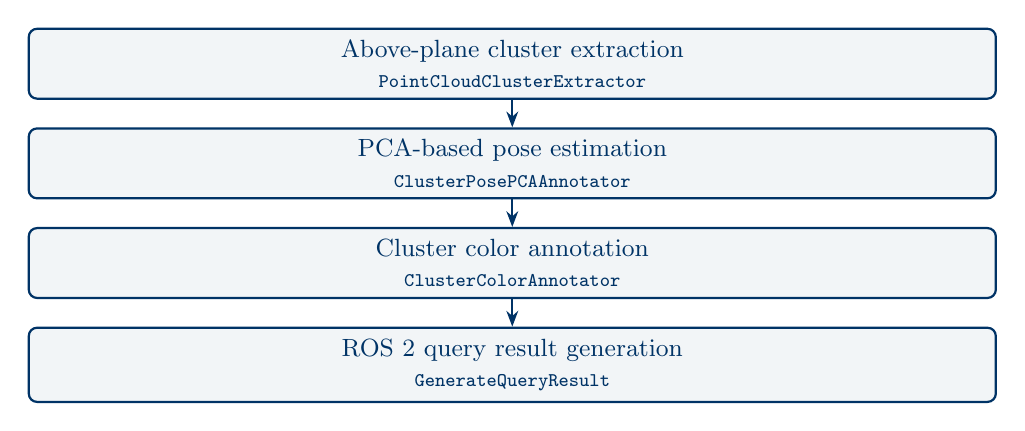
\begin{tikzpicture}[node distance=0.35cm]
    \node[pipeline step] (clusters) {Above-plane cluster extraction\\
      {\scriptsize\texttt{PointCloudClusterExtractor}}};
    \node[pipeline step, below=of clusters] (pose) {PCA-based pose estimation\\
      {\scriptsize\texttt{ClusterPosePCAAnnotator}}};
    \node[pipeline step, below=of pose] (color) {Cluster color annotation\\
      {\scriptsize\texttt{ClusterColorAnnotator}}};
    \node[pipeline step, below=of color] (result) {ROS 2 query result generation\\
      {\scriptsize\texttt{GenerateQueryResult}}};
    \draw[pipeline arrow] (clusters) -- (pose);
    \draw[pipeline arrow] (pose) -- (color);
    \draw[pipeline arrow] (color) -- (result);
  \end{tikzpicture}
\end{frame}

\begin{frame}{Observed behavior}
  The pipeline demonstrated the complete path from RGB-D acquisition to object
  hypotheses with pose and color information.

  \medskip
  The pipline was falsly ditecting large box of grey and white(for reflective areas) of the table.
  While missing requested colored cubes.
\end{frame}

\section{Blue}

% %% Blue pipeline flowchart
\begin{frame}{Preception Pipline 2: Blue(1/2)}
  \centering
  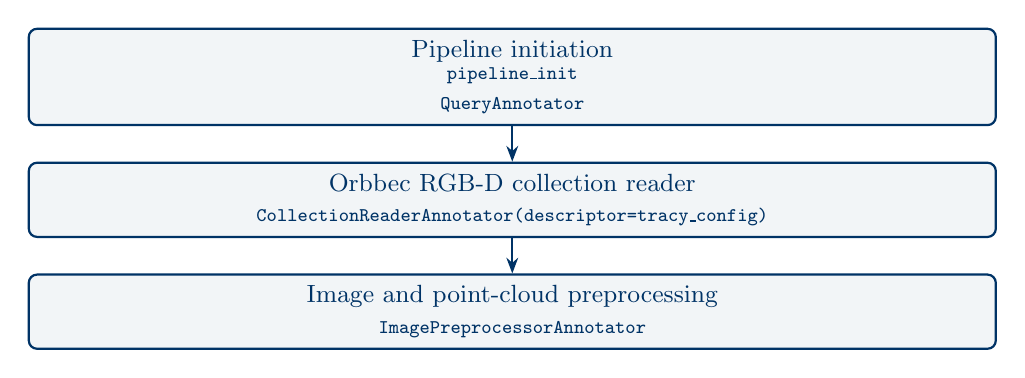
\begin{tikzpicture}[node distance=0.45cm]
    \node[pipeline step] (initiation) {Pipeline initiation\\
      {\scriptsize\texttt{pipeline\_init}\\\texttt{QueryAnnotator}}};
    \node[pipeline step, below=of initiation] (reader) {Orbbec RGB-D collection reader\\
      {\scriptsize\texttt{CollectionReaderAnnotator(descriptor=tracy\_config)}}};
    \node[pipeline step, below=of reader] (preprocessing) {Image and point-cloud preprocessing\\
      {\scriptsize\texttt{ImagePreprocessorAnnotator}}};
    \draw[pipeline arrow] (initiation) -- (reader);
    \draw[pipeline arrow] (reader) -- (preprocessing);
  \end{tikzpicture}
  \par\smallskip
  {\scriptsize\color{uniblue}Continues with query-selected HSV segmentation.}
\end{frame}

\begin{frame}{Preception Pipline 2: Blue(2/2)}
  \centering
  {\scriptsize\color{uniblue}From image and point-cloud preprocessing.}
  \par\smallskip
  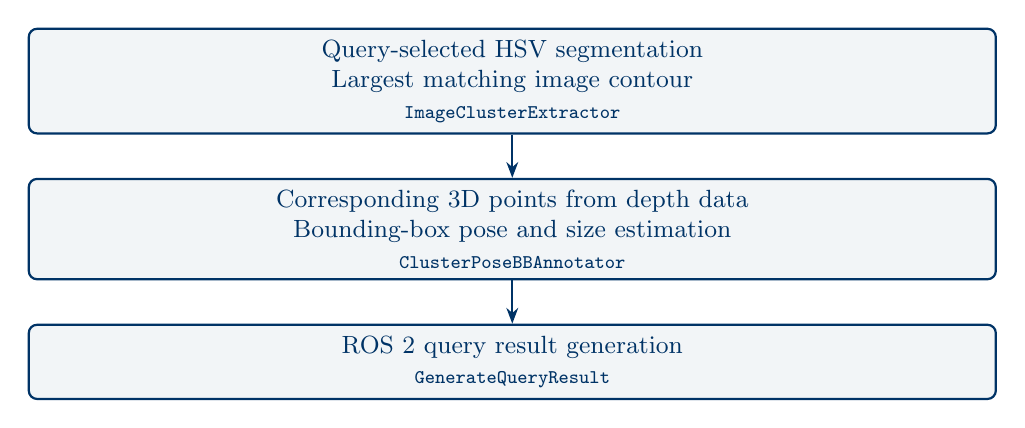
\begin{tikzpicture}[node distance=0.55cm]
    \node[pipeline step] (segmentation) {Query-selected HSV segmentation\\
      Largest matching image contour\\
      {\scriptsize\texttt{ImageClusterExtractor}}};
    \node[pipeline step, below=of segmentation] (pose) {Corresponding 3D points from depth data\\
      Bounding-box pose and size estimation\\
      {\scriptsize\texttt{ClusterPoseBBAnnotator}}};
    \node[pipeline step, below=of pose] (result) {ROS 2 query result generation\\
      {\scriptsize\texttt{GenerateQueryResult}}};
    \draw[pipeline arrow] (segmentation) -- (pose);
    \draw[pipeline arrow] (pose) -- (result);
  \end{tikzpicture}
\end{frame}

\begin{frame}{Observed behavior}
  In the performed demonstrations, this pipeline reliably detected the queried
  colored cube and returned its bounding-box pose.

  \medskip
  It precisly ditect even the pose of smaller cubes.

  \medskip
  It provided the perception
  output required by the subsequent CRAM/Coraplex integration.
\end{frame}

\section{Storage Red}

% %% Storage Red motivation and comparison
\begin{frame}{Storage Red: why MCAP?}
  \begin{itemize}
    \setlength{\itemsep}{0.9cm}
    \item \textbf{Motivation:} On the newer Linux kernel used for this project,
      the original RoboKudo MongoDB recording workflow encountered a
      compatibility problem.
    \item \textbf{Response:} \texttt{storage\_red.py} is a dedicated RoboKudo
      analysis engine with a \texttt{McapRecorderAnnotator}. It records the
      sensor input needed to reproduce a perception run in an MCAP bag.
  \end{itemize}
\end{frame}

\begin{frame}{Storage Red: previous and current recording}
  \centering
  \footnotesize
  \setlength{\tabcolsep}{4pt}
  \renewcommand{\arraystretch}{1.4}
  \begin{tabular}{|>{\raggedright\arraybackslash}p{2.4cm}|>{\raggedright\arraybackslash}p{4.8cm}|>{\raggedright\arraybackslash}p{5.5cm}|}
    \hline
    \textbf{Aspect} & \textbf{Previous: \texttt{storage.py}} & \textbf{New: \texttt{storage\_red.py}} \\
    \hline
    Storage backend & MongoDB through \texttt{StorageWriter} & ROS 2 rosbag2 with MCAP through \texttt{McapRecorderAnnotator} \\
    \hline
    Data saved & Processed CAS data, views, and world model state & Original RGB-D, camera-info, and transform ROS messages \\
    \hline
    Recording behavior & Writes the current CAS when the pipeline ticks & Records subscribed ROS topics continuously while the pipeline runs \\
    \hline
    Replay input & MongoDB records read back into a CAS & MCAP bag replayed as sensor topics \\
    \hline
    Advantage in the notes & More compressed & Easier implementation \\
    \hline
  \end{tabular}
\end{frame}

% %% Storage Red recording flow and topics
\begin{frame}{Storage Red: processing flow}
  \centering
  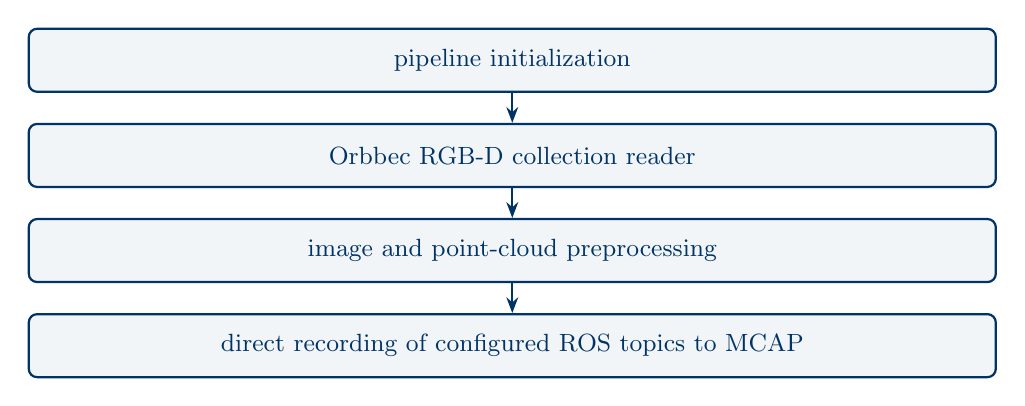
\begin{tikzpicture}[node distance=0.38cm]
    \node[pipeline step] (initiation) {pipeline initialization};
    \node[pipeline step, below=of initiation] (reader) {Orbbec RGB-D collection reader};
    \node[pipeline step, below=of reader] (preprocessing) {image and point-cloud preprocessing};
    \node[pipeline step, below=of preprocessing] (recording) {direct recording of configured ROS topics to MCAP};
    \draw[pipeline arrow] (initiation) -- (reader);
    \draw[pipeline arrow] (reader) -- (preprocessing);
    \draw[pipeline arrow] (preprocessing) -- (recording);
  \end{tikzpicture}
\end{frame}

\begin{frame}{Storage Red: recorded topics}
  \centering
  \footnotesize
  \setlength{\tabcolsep}{4pt}
  \renewcommand{\arraystretch}{1.45}
  \begin{tabular}{|>{\raggedright\arraybackslash}p{3.4cm}|>{\raggedright\arraybackslash}p{3.1cm}|>{\raggedright\arraybackslash}p{6.2cm}|}
    \hline
    \textbf{Topic source} & \textbf{Recorded information} & \textbf{Purpose during replay} \\
    \hline
    Orbbec depth topic & Depth image & Reconstruct three-dimensional scene data \\
    \hline
    Orbbec color topic & RGB image & Run color-based image processing \\
    \hline
    Orbbec camera-info topic & Camera calibration & Interpret and project image measurements \\
    \hline
    \texttt{/tf\_static} & Static transforms & Recover fixed sensor-frame relationships \\
    \hline
  \end{tabular}
\end{frame}

\section{MCAP recorder}

% %% MCAP recorder lifecycle
\begin{frame}{MCAP recorder: lifecycle (1/2)}
  \centering
  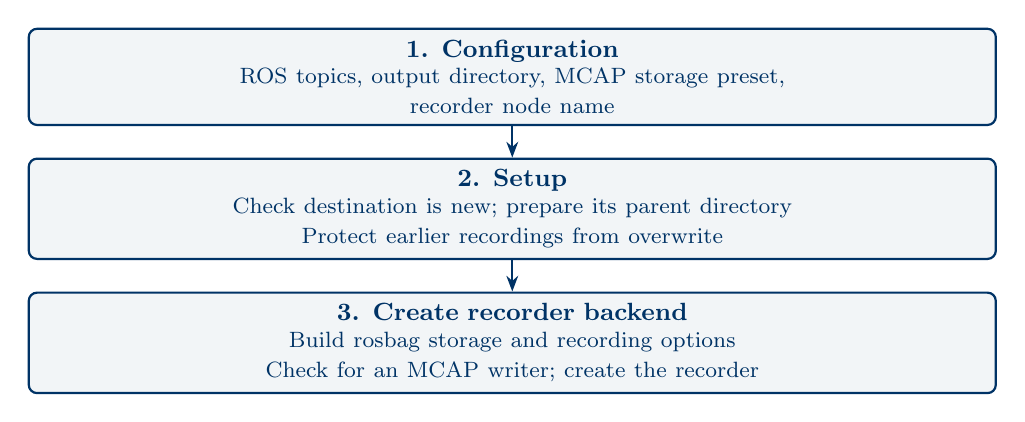
\begin{tikzpicture}[node distance=0.4cm]
    \node[pipeline step] (configuration) {\textbf{1. Configuration}\\
      {\footnotesize ROS topics, output directory, MCAP storage preset,\\recorder node name}};
    \node[pipeline step, below=of configuration] (setup) {\textbf{2. Setup}\\
      {\footnotesize Check destination is new; prepare its parent directory\\Protect earlier recordings from overwrite}};
    \node[pipeline step, below=of setup] (backend) {\textbf{3. Create recorder backend}\\
      {\footnotesize Build rosbag storage and recording options\\Check for an MCAP writer; create the recorder}};
    \draw[pipeline arrow] (configuration) -- (setup);
    \draw[pipeline arrow] (setup) -- (backend);
  \end{tikzpicture}
  \par\smallskip
  {\scriptsize\color{uniblue}Continues with continuous recording.}
\end{frame}

\begin{frame}{MCAP recorder: lifecycle (2/2)}
  \centering
  {\scriptsize\color{uniblue}From recorder backend creation.}
  \par\smallskip
  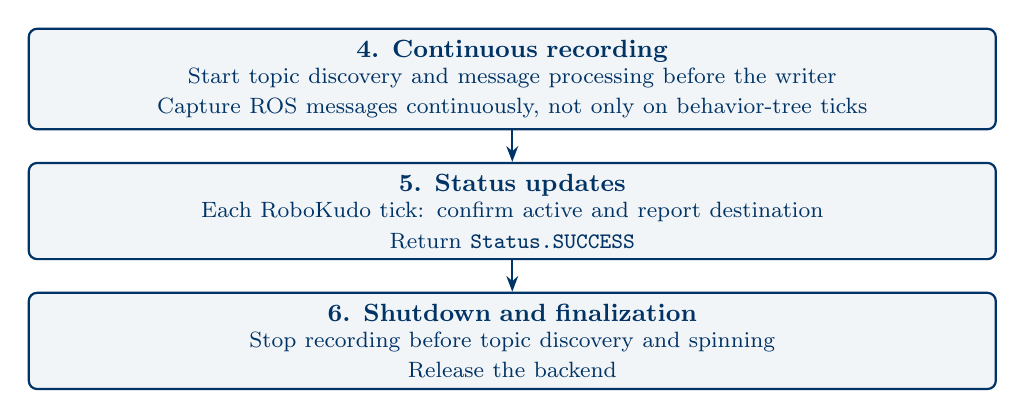
\begin{tikzpicture}[node distance=0.4cm]
    \node[pipeline step] (recording) {\textbf{4. Continuous recording}\\
      {\footnotesize Start topic discovery and message processing before the writer\\Capture ROS messages continuously, not only on behavior-tree ticks}};
    \node[pipeline step, below=of recording] (status) {\textbf{5. Status updates}\\
      {\footnotesize Each RoboKudo tick: confirm active and report destination\\Return \texttt{Status.SUCCESS}}};
    \node[pipeline step, below=of status] (shutdown) {\textbf{6. Shutdown and finalization}\\
      {\footnotesize Stop recording before topic discovery and spinning\\Release the backend}};
    \draw[pipeline arrow] (recording) -- (status);
    \draw[pipeline arrow] (status) -- (shutdown);
  \end{tikzpicture}
\end{frame}

\begin{frame}{MCAP recorder: observed behavior}
  \begin{itemize}
    \setlength{\itemsep}{0.55cm}
    \item The analysis engine recorded the configured sensor stream to an MCAP bag.
    \item The data was replayed successfully.
    \item Many later experimantations was done using the data stored next cloud using storage red.
  \end{itemize}

  \bigskip
  \centering
  \textcolor{uniblue}{\textbf{Laptop demonstration: replay the MCAP bag.}}
\end{frame}

\section{CRAM and RoboKudo Integration}

% %% CRAM integration query flow
\begin{frame}{CRAM and RoboKudo integration V1}
  \centering
  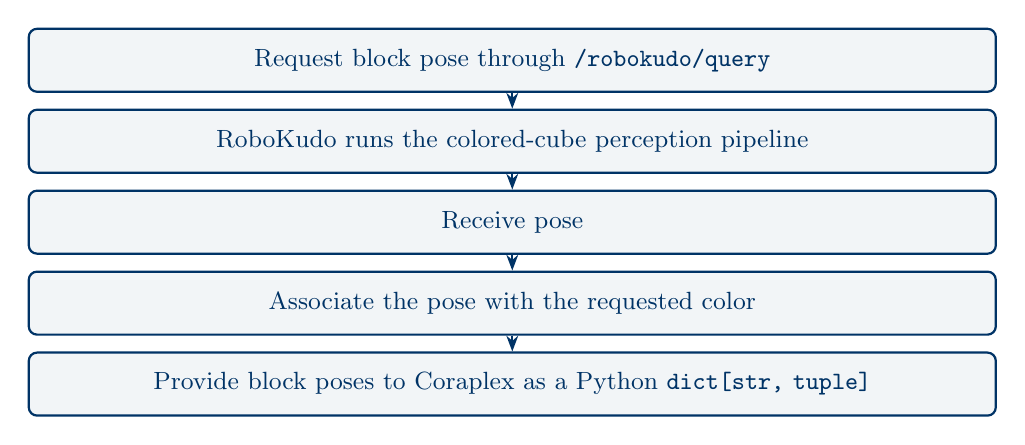
\begin{tikzpicture}[node distance=0.2cm]
    \node[pipeline step] (request) {Request block pose through \texttt{/robokudo/query}};
    \node[pipeline step, below=of request] (perception) {RoboKudo runs the colored-cube perception pipeline};
    \node[pipeline step, below=of perception] (pose) {Receive pose};
    \node[pipeline step, below=of pose] (color) {Associate the pose with the requested color};
    \node[pipeline step, below=of color] (task) {Provide block poses to Coraplex as a Python \texttt{dict[str, tuple]}};
    \draw[pipeline arrow] (request) -- (perception);
    \draw[pipeline arrow] (perception) -- (pose);
    \draw[pipeline arrow] (pose) -- (color);
    \draw[pipeline arrow] (color) -- (task);
  \end{tikzpicture}
  \par\smallskip
  {\scriptsize\color{uniblue}Block-stacking integration without SemDtSync.}
\end{frame}

\begin{frame}{CRAM and RoboKudo: query behavior}
  \begin{itemize}
    \setlength{\itemsep}{0.5cm}
    \item \textbf{White pipeline:} Estimates all block poses at the same time in
      one perception pipeline run.
    \item \textbf{Blue pipeline:} Each ROS action goal requests object type
      \texttt{block} and one requested color. Found colors are retained; missing
      colors are queried again using a fresh perception result, up to the
      attempt limit.
    \item \textbf{Action-future handling:} The query works with a standalone ROS
      node and with a node already managed by an executor.
  \end{itemize}
\end{frame}

\end{document}
